\chapter{Development workflow in CEDRE}

  \paragraph{}
  In this brief chapter, we will discuss the details of how we implemented selected methods in CEDRE.
  This does not constitute research work, but it ended up being a large part of the work done during this thesis.
  It is also not without interest, as we sometimes used advanced features in order to implement what we set out to do.


  \section{Description of CEDRE}

    \paragraph{}
    The software system CEDRE gather several solvers to solve problems in the field of multiphysics \cite{ReflochCourbetMurroneEtAl2011}.
    Each solver is dedicated to a given model.
    As of today, there are seven solvers embedded in CEDRE:
    \begin{itemize}
      \item CHARME, the fluid solver, for compressible multifluid and reactive flow, with RANS or LES turbulence models
      \item SPIREE, the dispersed phase solver using an Eulerian framework
      \item SPARTE, the dispersed phase solver using a Lagrangian framework
      \item ASTRE, the radiation solver using a Monte Carlo method
      \item REA, the radiation solver using a discrete ordinates method
      \item FILM, for shallow water equations, used to model ice accretion
      \item ACACIA, the conduction solver, for heat transfer in solids.
    \end{itemize}
    Combining different solvers, CEDRE is able to simulate multiphysics phenomena numerically.
    Using those solvers, CEDRE applications go from aerodynamics to aeroacoustics, aerothermodynamics, combustion, icing, etc.
    The solver is coupled either through boundary conditions for example in a thermal interaction at a fluid-structure contact or inside the computational domain for example in the case of mass and energy transfer between dispersed phases and the main flow.
    The coupling can either be one-way or two-way, depending on the user's choice.
    Each solver is integrated in time separately, and the coupling consists of some data exchange between iterations: it is an explicit coupling.

    \paragraph{}
    Some functionalities common to multiple solvers exist outside the solver in helper libraries.
    For instance:
    \begin{itemize}
      \item ASSEMBLAGE acts as the conductor by handling the overall simulation, telling the solvers what to do and when to do it, when to exchange data and with which other coupled solver
      \item BIBCEDRE contains tools for geometrical operations, linear algebra methods, mesh handling, parallel communications and other general functionalities
      \item THERMOLIB is used to compute the different thermophysical properties such as heat capacities, chemical reaction rates, etc. \PS{Lionel je dis pas de bêtise sur les coefficients de réaction chimique ?}
    \end{itemize}
    Those libraries are the main engines of the solver.
    When we do a computation with CHARME, it is in fact ASSEMBLAGE that tells CHARME when to initialise itself, to do a step of the time integration method, etc.
    When CHARME needs to compute the ordinary differential equation function, it is BIBCEDRE that does the MUSCL reconstruction \PS{c'est bien ça ?} so that the Riemann solver can compute the interface flux.
    When CHARME needs to compute the primitive variables such as the pressure and temperature from the conservative variables, it is THERMOLIB that solves a nonlinear problem with Newton's method to compute the result.

    \paragraph{}
    Now that we defined the existing framework for the software system CEDRE, we can develop new functionalities.
    Despite allowing some flexibility in the programming language, most of CEDRE is written in Fortran.
    We decided to keep working with Fortran to help with the integration of our work.
    As CEDRE is used by industrial clients, and as they rely on their own supercomputers, we need to limit ourselves to Fortran 2003 standards, so as to ensure compatibility.


  \section{Implementation details}


    \paragraph{}
    In this thesis, we focused on the most used solver: CHARME.
    Indeed, not only is it the most used, but other solvers use it as a base for many applications.
    For example, when simulating ice accretion around a wing profile, a standard methodology with CEDRE is to first get the base aerodynamic flow with CHARME and then compute the ice particles with SPIREE or SPARTE.
    Working with the solver CHARME was the way to benefit the most from our work.
    Even if during this thesis we only worked on CHARME, we always kept in mind that the finality was multiphysics simulations using multiple solvers.
    That is why we tried to develop generic functionalities so that they could be easily imported to other solvers, provided the developers of said solvers wanted to use them.
    The same reason was also used as a criterium in our choices, as was explained previously.
    Choosing the Jacobian-Free Newton--Krylov method goes towards fully implicit coupling between solvers, instead of the explicit coupling existing today.

    \subsection{FGMRES}

      \paragraph{}
      In order for our work to be usable in every other solver, we had to work on the common library BIBCEDRE.
      When the implicit Euler method of CHARME needs to solve a linear problem, it uses BIBCEDRE.
      It contains everything needed to solve linear problems, such as GMRES and preconditioners.
      A linear problem is stored in BIBCEDRE as the Fortran derived type \mintinline{fortran}{type_sys}.
      In order to add Flexible preconditioning to the existing GMRES, we added a pointer to an inner instance of \mintinline{fortran}{type_sys} inside of \mintinline{fortran}{type_sys}, so that the linear system and its corresponding solver may use an inner solver for an inner problem:
\begin{minted}{fortran}
  type type_sys
    ! Inner linear system and solver
    type(type_sys), pointer :: sys_int => null()

    ... ! Additional data
  end type type_sys
\end{minted}
      This way, when we need to apply the preconditioner during a GMRES iteration, we can use the inner \mintinline{fortran}{type_sys} instance to call the inner GMRES.
      Furthermore, having a pointer to an inner instance allows for more freedom for the inner solver.
      One could for instance use multiple depths of preconditioning and have the inner GMRES also be an FGMRES method, preconditioned by another GMRES, etc.


    \subsection{Matrix-free}

      \paragraph{}
      Sparse matrices are stored in an in-house format, using an array for the diagonal blocks, another one for the extra-diagonal blocks and a third one to index the extra-diagonal blocks.
      Matrix vector products are made inside BIBCEDRE to handle this matrix format, with the routine:
\begin{minted}{fortran}
  subroutine gmvec(sys, i_p, i_ap)
    type(type_sys), intent(inout) :: sys
    integer,        intent(in)    :: i_p
    integer,        intent(in)    :: i_ap
\end{minted}
      that takes three arguments: the \mintinline{fortran}{type_sys} instance, an index identifying the vector to multiply and an index identifying the vector where to put the result.
      As we explained when we introduces Krylov subspace methods, GMRES uses the linear system matrix through this matrix vector product routine.
      Classically, a client solver such as CHARME fills the matrix coefficients and then lets BIBCEDRE solve the linear system.
      In order to use the matrix-free approximation from equation (\ref{eq:matrix_free}), we only need to replace this routine with a new one that computes the approximation.
      Unfortunately, the approximation uses a function that belongs to the client solver.
      The library BIBCEDRE does not know this function and how to compute it, as it is part of CHARME or any other client solver.
      As we said, we want to write generic solutions, and so merging the library BIBCEDRE with the solver CHARME is not a good solution.
      What we need here is to allow BIBCEDRE to use a callback from the client solver.
      We did that using the Fortran 2003 feature: polymorphism.
      The Fortran 2003 standard is almost ten years old as of today, and many may consider that the functionalities added to the previous Fortran 95 standard are therefore not that innovative.
      But in the context of a project as large as CEDRE, developed by researchers and used by industrial partners, even the Fortran 2003 standard and polymorphism in particular are innovative.
      Without going into too much detail, we added a member to the type \mintinline{fortran}{type_sys} that contains the context to evaluate a matrix-vector product:
\begin{minted}{fortran}
  type type_sys
    ! Matrix vector product context
    class(type_gmvec_ctx), pointer :: gmvec_ctx => null()

    ... ! Additional data
  end type type_sys
\end{minted}
      with:
\begin{minted}{fortran}
  type type_gmvec_ctx
    procedure(interface_gmvec), pointer, nopass :: gmvec

    ... ! Additional data
  end type type_gmvec_ctx
\end{minted}
      This way, when the client solver creates an instance \mintinline{fortran}{sys} of \mintinline{fortran}{type_sys}, it can choose how to evaluate matrix-vector products by setting the procedure pointer \mintinline{fortran}{sys%gmvec_ctx%gmvec}.
      It can for example point to the already existing routine to use the classical matrix-vector product, but it also can use a custom routine that implements the approximation (\ref{eq:matrix_free}).
      Furthermore, the client solver can use polymorphism and create an extended type of \mintinline{fortran}{type_gmvec_ctx} in order to store additional data in the context.
      This is what is done by the solver CHARME, as it does need additional data to approximate the Jacobian matrix-vector product.
      Finally, with this implementation, any solver that wants to use the approximation (\ref{eq:matrix_free}) just needs to write the corresponding routine and set the context accordingly.
      Then, a user can choose at execution time whether to use the standard Jacobian matrix or the matrix-free method.

      \paragraph{}
      The computational cost of the matrix-vector approximation is approximately the cost of one function evaluation.
      It requires some additional operations, such as vector subtractions, and vector scaling, but those operations are way less expensive.
      Using a matrix-free algorithm is clearly less expensive in terms of memory, as we do not need to store the matrix at all.
      Some even claim that it can lead to a less expensive method in terms of time \cite{AnWenFeng2011}.
      This happens when the alternative, which is computing the Jacobian matrix, is an expensive task.
      In CHARME, the Jacobian matrix that is traditionally used is inexpensive to compute, with a cost similar to a function evaluation.
      The issue is that the function evaluation itself is expensive in our solver.
      This is troublesome, and the issue is currently addressed by the team of developers in charge of the solver.
      In the meantime, it means that the cost of the matrix-free approximation will suffer even more.
      Practically, using it increases the computational time of one iteration.
      We now hope that as it will not improve the iteration speed, it will improve the convergence of our solver.
      Also, as we said the team responsible for CEDRE is working to improve the speed of the function evaluation.
      If they succeed, our method will then benefit greatly from their work.


    \subsection{Strategy for the choice of \texorpdfstring{$\varepsilon$}{epsilon}}
      \PS{Bouger cette partie ?}

      \paragraph{}
      When we introduced the approximation (\ref{eq:matrix_free}) we saw a new parameter $\varepsilon$.
      It is easy to check that the truncation error on this approximation decreases linearly with regard to $\varepsilon$.
      It is natural to take a small value for $\varepsilon$.
      But unfortunately, we work with floating-point arithmetic, so dividing by a small $\varepsilon$ introduces a roundoff error.
      This parameter needs to balance truncation and roundoff error.
      We need to decide on a strategy for the choice of epsilon.
      We could take for example $\varepsilon = \sqrt{\varepsilon_\textrm{mach}}$ where $\varepsilon_\textrm{mach}$ is the machine epsilon: around $10^{-6}$ for single precision and $10^{-15}$ for double precision.
      This choice is often discarded as it is deemed too simplistic.
      Instead, works from the literature tend to use the same few options \cite{ParkNourgalievMartineauEtAl2009, LiuZhangZhongEtAl2015, AbhyankarBrownConstantinescuEtAl2018} that come from \cite{PerniceWalker1998} and \cite{DennisSchnabel1996}.
      Those options are well described in \cite{KnollKeyes2004}.
      In particular, the one that we encounter the most is the one from \cite{PerniceWalker1998}:
      \begin{equation}\label{eq:epsilon_wp}
        \varepsilon_\textrm{wp} = \frac{\sqrt{\varepsilon_0 \left(1 + \norm[2]{x}\right) }}{\norm[2]{v}}
      \end{equation}
      using the same $x$ and $v$ as in equation (\ref{eq:matrix_free}).
      Here $\varepsilon_0$ is the estimated relative error in function evaluation.
      A reason this choice is so popular is that apart from this $\varepsilon_0$ value, it does not require any user input.
      Furthermore, $\varepsilon_0$ is often simply set to machine epsilon $\varepsilon_\textrm{mach}$.

      \paragraph{}
      To analyse this strategy in the choice of $\varepsilon$, we do the following numerical experiment.
      We consider the 1D Burgers' equation over a regular periodic mesh made of 10 cells (or segments in 1D).
      The function $f$ is taken as the right-hand side of equation (\ref{eq:ode}) when solving the Burgers' equation, using a first-order Finite Volume method as the spatial discretisation method, itself using an exact Riemann solver (Godunov's scheme).
      This function was chosen because it is a nonlinear conservative equation, often viewed in computational fluid dynamics as a simplified version of Euler equations and it contains most aspects of nonlinear hyperbolic equations.
      The vectors $x$ and $v$ are $10 + r_1$ and $0.1 \left(2 r_2 - 1\right)$ where $r_1$ and $r_2$ are random vectors following a uniform distribution on $\left[0, 1\right[$, obtained with the Python package NumPy: \mintinline{python}{numpy.random.random}.

      \begin{figure}
        \centering
        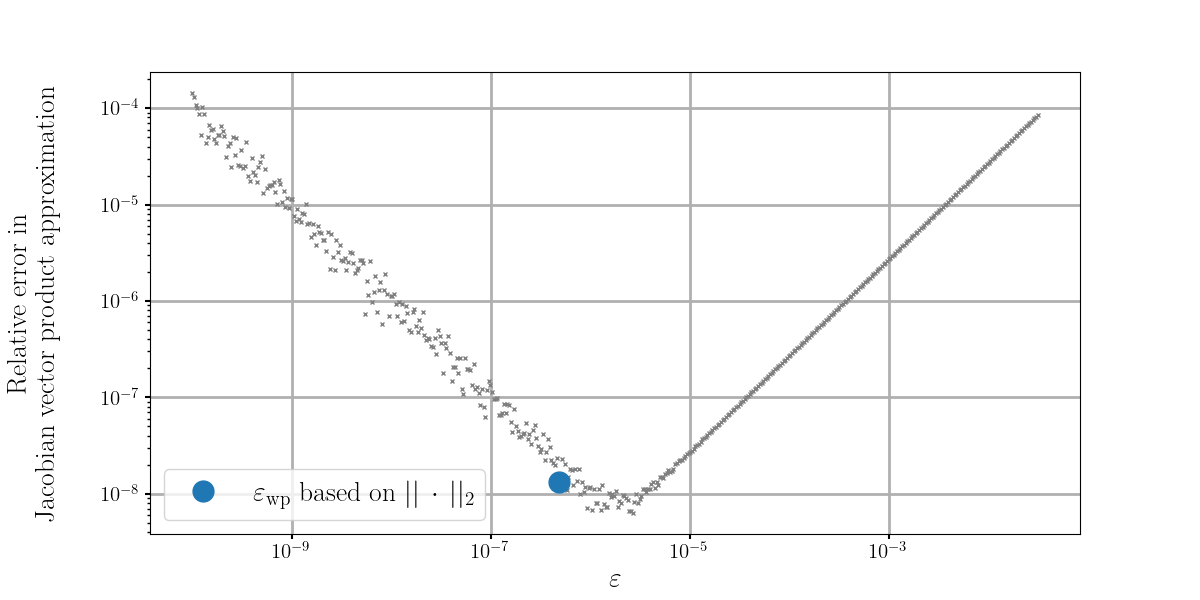
\includegraphics[width=\textwidth]{figures/epsilon_Burgers_10.png}
        \caption{
          Error in the Jacobian matrix-vector product approximation as a function of $\varepsilon$, and in particular for the most popular choice $\varepsilon_\textrm{wp}$.
          The function is the right-hand side of equation (\ref{eq:ode}) from a Finite Volume method using an exact Riemann solver for Burgers' equation, over a 10-cell 1D regular mesh.
        }
        \label{fig:epsilon_burgers_10}
      \end{figure}

      \paragraph{}
      The experiment result can be seen in figure \ref{fig:epsilon_burgers_10}.
      The relative error in the approximation is shown as a function of $\varepsilon$ with small grey crosses.
      On the right part of the figure, the error decreases linearly with regard to $\varepsilon$.
      This corresponds to a truncation error-dominated region.
      On the left part, the error increases as $\varepsilon$ decreases.
      This corresponds to a roundoff error-dominated region.
      Also, this increase is not smooth as the linear decrease, because roundoff errors tend to produce more chaotic results.
      The choice of $\varepsilon$ from \cite{PerniceWalker1998} is also shown in the figure, as the large blue dot.
      As we can see, it falls into a low error region, not too much on the left, not too much on the right.

      \paragraph{}
      The issue we noticed is the following.
      Some references in the literature do not specify the norm used in equation (\ref{eq:epsilon_wp}).
      As it is most of the time the Euclidian norm $\norm[2]{\,\cdot\,}$, or 2-norm, we can assume that it is also the case when it is not specified.
      However, this means that in our example the value of $\varepsilon_\textrm{wp}$ will depend on the vector size.
      With our example, if we increase the number of cells in our mesh the typical size of the vector components stays roughly the same, so the shape of the error as a function of $\varepsilon$ should not change much from the one in figure \ref{fig:epsilon_burgers_10}.
      But if the vector components size stays the same, the 2-norm does increases with the vector dimension.
      We can even see that when the dimension is $N \gg 1$, $\varepsilon_\textrm{wp} \sim N^{-1/4}$.
      Having $\varepsilon$ to depend on $N$ did not make sense to us, as we are working with possibly large vectors in our industrial applications.
      That is why we decided to use a variation from what is currently found in the literature: we will use the norm $\norm[2]{\,\cdot\,} / \sqrt{N}$ that can be seen as a scaled 2-norm.
      We then get a new strategy for the choice of $\varepsilon$ that we note $\varepsilon_{\textrm{wp}, N}$:
      \begin{equation}
        \varepsilon_{\textrm{wp}, N} = \frac{\sqrt{\varepsilon_0 \left(1 + \norm[2]{x} / \sqrt{N}\right) }}{\norm[2]{v} / \sqrt{N}} \ .
      \end{equation}

      \begin{figure}
        \centering
        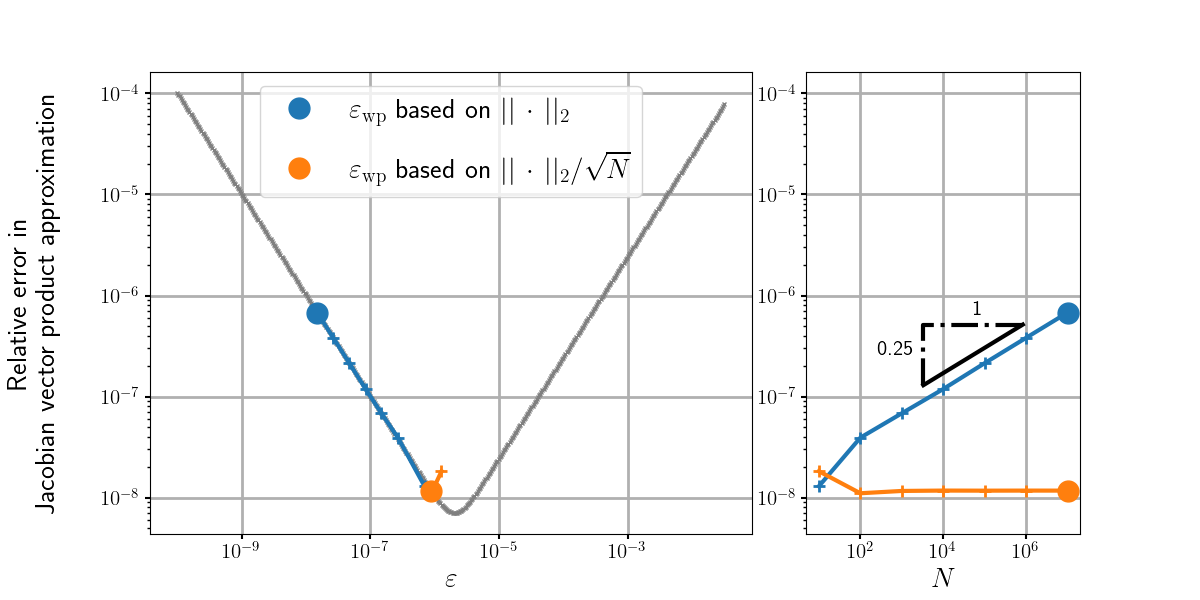
\includegraphics[width=\textwidth]{figures/epsilon_Burgers.png}
        \caption{
          Error in the Jacobian matrix-vector product approximation as a function of $\varepsilon$ (left) and of the dimension $N$ (right).
          On the left figure, coloured cross markers correspond to the values computed on a mesh of $10^1$, $10^2$, ... cells, and circle markers to the last value with $10^7$ cells.
          Grey cross markers on the left figure correspond to a mesh of $10^7$ cells.
        }
        \label{fig:epsilon_burgers}
      \end{figure}

      \paragraph{}
      We compared the two strategies on the same test case while increasing the number of cells from 10 to 100, 1000, ..., up to $10^7$.
      Figure \ref{fig:epsilon_burgers} shows the result of this experiment.
      On the left, we see that the shape of the relative error as a function of $\varepsilon$ when $N = 10^7$ is similar to when $N = 10$, albeit the roundoff error-dominated region is more regular.
      In particular, the ideal trade-off between the two error types did not move a lot.
      We see that as expected, the value of $\varepsilon_\textrm{wp}$ decreases: this translate as the fact that the blue dot moved to the left.
      When looking at the error as a function of the dimension $N$, we can even recover the $-1/4$ expected slope.
      In the right figure, we see in fact a $1/4$ slope but the error is inversely proportional to the value of $\varepsilon$ so if the error \PS{varie en} $N^{1/4}$, then $\varepsilon_\textrm{wp}$ \PS{varies in} $N^{-1/4}$.
      Because of the shape of the error as a function of $\varepsilon$, if $\varepsilon_\textrm{wp}$ changes with $N$ it will eventually end up increasing the error.
      This is an undesired feature.
      Our new choice $\varepsilon_{\textrm{wp}, N}$ on the other hand does not change a lot when $N$ increases.
      Therefore, the error level stays the same no matter the dimension.

      \paragraph{}
      The same numerical experiment was made on a more complex case: the 1D Euler equations.
      Here, the function $f$ corresponds to the right-hand side of equation (\ref{eq:ode}) given by a centred Finite Volume method used as the spatial discretisation method, in which the interface flux is defined as an average of left and right fluxes.
      This means the Riemann solver just averages the left and right fluxes.
      This spatial method is known for its instability when used in an actual solver, but it is useful in this experiment as the analytic Jacobian matrix is easy to derive, contrary to methods using more complex Riemann solvers.
      This physical model assigns 3 degrees of freedom in each cell.
      We will use primitive variables.
      The vector $x$ corresponds to a uniform density of $1\si{\kilogram\per\cubic\meter}$, a velocity equal to a sine making one period over the mesh and of amplitude $10\si{\meter\per\second}$, and uniform pressure of $10^5\si{\pascal}$.
      The vector $v$ is a random vector in $\left[0, 1\right]$ as before, where the first component is scaled by $10^{-3}$, the second by $10^{-2}$, and the third by $10^{2}$, in order to impose $10^{-3}$ relative perturbations.

      \begin{figure}
        \centering
        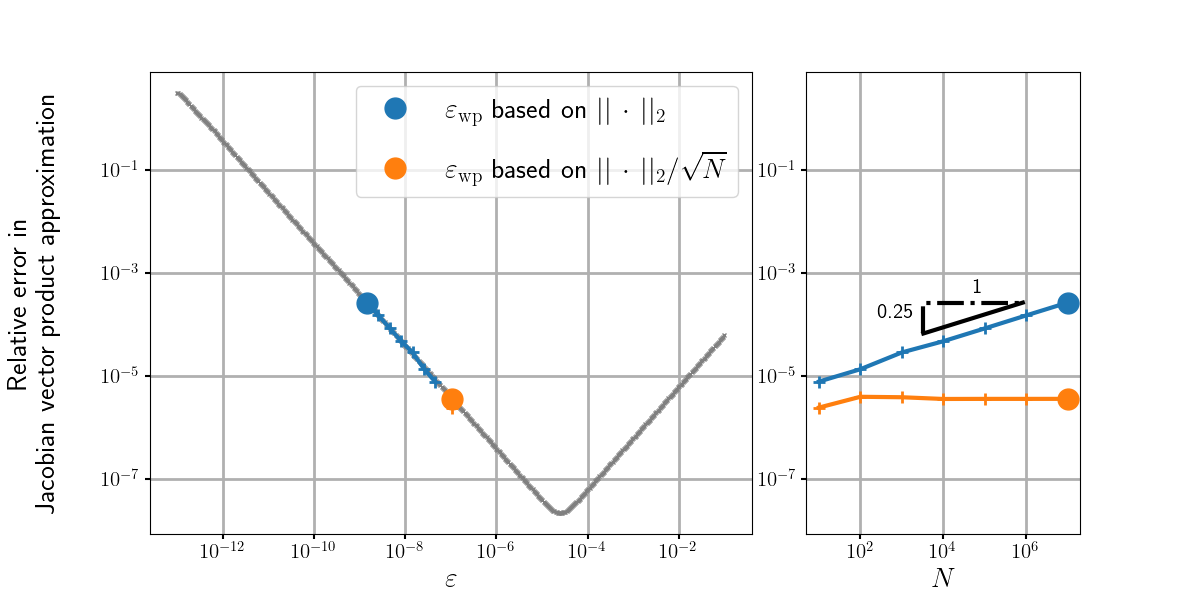
\includegraphics[width=\textwidth]{figures/epsilon_Euler.png}
        \caption{
          Error in the Jacobian matrix-vector product approximation as a function on $\varepsilon$ (left) and of the dimension $N$ (right).
          The function is the right-hand side of equation (\ref{eq:ode}) from a Finite Volume method using a centred scheme for the Euler equations over a regular 1D mesh.
          On the left figure, coloured cross markers correspond to the values computed on a mesh of $10^1$, $10^2$, ... cells, and circle markers to the last value with $10^7$ cells.
          Grey cross markers on the left figure correspond to a mesh of $10^7$ cells.
        }
        \label{fig:epsilon_euler}
      \end{figure}

      \paragraph{}
      Figure \ref{fig:epsilon_euler} shows the corresponding results.
      As for the previous experiment, $\varepsilon_\textrm{wp}$ depends on the dimension $N$, and then the associated error ends up increasing as $N$ grows.
      Our correction $\varepsilon_{\textrm{wp}, N}$ does not exhibit the same drawback.
      Even if it does not fall at the bottom of the error curve, it at least does not lead to a larger error.

      \paragraph{}
      In this last case, we see that at the beginning the two errors were close.
      In the first one, their starting positions were a bit different.
      This is largely due to the randomness of this analysis: the one used to construct the $x$ and $v$ vectors.
      In fact, it would be unwise to draw a conclusion from the position of the points in figures \ref{fig:epsilon_burgers} and \ref{fig:epsilon_euler}.
      Changing the choice of vectors, of the function $f$, or even the randomness in the vectors is enough to modify their position.
      For example, we can not conclude anything from the fact that $\varepsilon_\textrm{wp}$ is almost at the bottom of the error curve in figure \ref{fig:epsilon_burgers}.
      It may as well be a bit more on the side.
      What we can use from this analysis, however, is the tendencies that choices of $\varepsilon$ show.
      The main conclusion is then that with our strategy we removed a dependency of the relative error on the dimension, which makes sense as this dependency is not expected a priori.

      \paragraph{}
      The issue with this analysis is that it relies on extremely simple examples.
      The function $f$ in our actual applications is in fact much more complicated than the two we used here.
      But in order to do this analysis we need to be able to compute the relative error, and this means we need to be able to compute a Jacobian matrix-vector product analytically.
      Unfortunately, this is not possible for our applications.
      If it was, we would not even need to introduce the approximation (\ref{eq:matrix_free}) and therefore do this analysis.
      Using Burgers' equation and 1D Euler equations with a simple Riemann solver was then a good compromise.
      Those equations share similarities with the ones we work with in our solver, as they are nonlinear hyperbolic equations, but they are still simple enough so that we can use them here.


    \subsection{Linear system normalisation}

      \PS{$N$ était utilisé comme taille des vecteurs juste au dessus, tant pis ?}

      \paragraph{}
      An available option in BIBCEDRE for the linear solve is normalisation.
      It consists in taking an invertible diagonal matrix $N$ and rewriting the linear system (\ref{eq:linear}) as:
      \begin{equation}
        \tilde{A}\tilde{x} = \tilde{b}
        \quad\textrm{with}\quad \tilde{A} = N^{-1} A N,
        \quad \tilde{x} = N^{-1} x
        \quad\textrm{and}\quad \tilde{b} = N^{-1} b \
      \end{equation}
      One can check that it is equivalent to the original linear system.
      The diagonal coefficients of the matrix $N$ are the invert of an estimate of the order of magnitude of the corresponding degree of freedom. \PS{clair ? beaucoup de of}
      This estimation can be computed at each time step depending on the current state, or can simply be constant equal to some reference values, depending on the choice of the user.
      When working with Euler equations, for example, the numerical values corresponding to the energy degrees of freedom are usually many orders of magnitudes over other degrees of freedom.
      The goal of this normalisation is to bring back each vector component at the same level in the linear system.
      It can also be seen as a combination of a left preconditioning by $N^{-1}$ and a right preconditioning by $N$.
      This normalisation is often used by our solver's users, so we need to ensure compatibility with our matrix-free method.
      We can adapt the approximation (\ref{eq:matrix_free}) to account for the normalisation as:
      \begin{equation}
        \left( N^{-1} f'\left(x\right) N \right) v \approx N^{-1} \frac{f\left(x + \varepsilon N v\right) - f\left(x\right)}{\varepsilon} \ .
      \end{equation}
      We also need to adapt our strategy for the choice of $\varepsilon$.
      With the normalisation, we see that $N \varepsilon$ sort of plays the role of $\varepsilon$.
      It then makes sense to take $\norm{N \varepsilon}$ equal to the original choice of $\varepsilon$, and therefore we take:
      \begin{equation}
        \varepsilon = \frac{\sqrt{\varepsilon_0 \left(1 + \norm{x}\right) }}{\norm{N} \norm{v}} \ .
      \end{equation}
      We take as a matrix norm the one induced by the vector norm.
      This means that:
      \begin{equation}
        \norm{N} = \sup_{v \ne 0} \frac{\norm{Nv}}{\norm{v}} \ .
      \end{equation}
      When using the 2-norm, the corresponding norm is $\norm{N} = \max{N_{ii}}$ as N is diagonal with strictly positive coefficients.
      When using the scaled 2-norm discussed in the previous part, the corresponding norm is also the same.
      This is nice because whatever strategy we use in the choice of $\varepsilon$, it does not interfere with the handling of normalisation.
      \PS{Par contre c'est en effet la théorie mais en pratique j'ai oublié de l'implémenter comme ça dans CEDRE, et on utilise la norme de Frobenius normalisée par la taille des vecteurs. Oups.}


    \subsection{Preconditioning}

      \paragraph{}
      Our matrix-free implementation also needs to be compatible with the already existing preconditioning from BIBCEDRE.
      There are two ways to precondition the linear system in BIBCEDRE.
      \begin{itemize}
        \item The \emph{outer} left preconditioning is applied once before the linear solve.
          It changes the numerical values of the matrix coefficients and of the right-hand side.
          Once it is applied, the solve can continue as if nothing had happened.
        \item The \emph{inner} right preconditioning is applied before each matrix-vector product, and once more at the end of the solve.
      \end{itemize}
      Handling the inner preconditioning with our matrix-free implementation is easy as those two operations are independent of each other.
      The outer preconditioning relies on the fact that the preconditioners available are simple, and therefore it is inexpensive to apply it to the whole matrix, and less expensive than applying after each matrix-vector product.
      We lose this advantage with our matrix-free method.
      We still apply once the left preconditioning to the right-hand side before the solve, but we now need to apply it after each matrix vector approximation.


    \subsection{Local time-stepping}

      \paragraph{}
      We said earlier that local time-stepping is used in CEDRE to accelerate the convergence on steady problems.
      What it does is that each cell of the mesh moves forward in time with its own time step, independently of other cells.
      This local time step is expressed as a fraction of the global time step.
      There are several options a user can choose from to set the time-stepping strategy.
      It can use CFL number based option and compute the corresponding local time step so that the CFL number local to the cell is not too large.
      The preferred and default option is based on the explicit increment and some reference values.
      It first estimates what the solution increment will be by using the explicit increment and possibly the reference values, depending on the choice of method, and compute a local time step so that the increment local to the cell is not too large.
      This local time-stepping strategy adds various parameters that need to be tuned, in the form of scalar coefficients, whether or not to apply the local time-stepping to the boundaries, whether to use conservative or primitive variables, etc.
      In the end, what local time-stepping methods do is artificially modify the volume of the cells: increasing a cell volume corresponds to increasing its inertia, and therefore scaling the time step down.
      The volumes of the cells appear in the linear system matrix, in the form of a diagonal "mass" matrix.
      By using the scaled mass matrix, the matrix-free approximation does account for local time-stepping.
      With this last feature, we ensured that the matrix-free approximation is compatible with the already existing methods.


  \paragraph{}
  This chapter explained in a simplified manner some implementation detail of our solver.
  It is important to remind oneself that CEDRE is an industrial-sized software system, compared to smaller solvers developed for academic purposes.
  The scale of the solver was a limiting factor in this thesis.
  We often wanted to try some new scientific idea but were faced with many troubles that are inherent to the solver size.
  At some point at the early stage of this thesis, for example, we wanted to improve the quality of the linear solve by using advanced solvers and preconditioners, with the help of the PETSc library \cite{petsc-web-page, petsc-user-ref, petsc-efficient}.
  Using the library in CEDRE ended up being impractical, or at least would have taken too much time that we could not afford, and so we had to change direction.
  In the end, a solver of this size is not an ideal sandbox to try methods that art too innovative.
  A good amount of experience is required to master the various models and methods, an amount I did not have at the beginning of this thesis.
  For example, the spatial discretisation methods come with a lot of parameters: the kind of method, the slope limiter, the Riemann solver, and many more that are specific to CEDRE.
  The same goes for the time integration with for instance the local time-stepping or the linear system normalisation.
  A single parameter may be deterministic in the success of a computation.
  This forces us to allocate a quite large amount of time to every computation.
  Moreover, because of the large number of developers that are working on the solver, and the fact that many developments are small tweaks from occasional developers such as interns and PhD students, fixing bugs also took a decent amount of time.
  Overall, this explains why we decided to implement the solutions previously discussed.
  They are already well known from the literature and feel like a natural step up from the already existing methods of CEDRE.
  It is good to mention that many difficulties arise from the solver, and are inherent to it, mostly due to its overall size.
  We would probably have taken a different route if we had worked with a different solver.


  \paragraph{}
  Without getting into too much detail, this chapter explained how the selected methods and modifications were implemented into the solver CEDRE.
  Besides some minor developments, the main feature is the matrix-free implementation.
  As it was explained, this implementation is generic so that it can be used with any solver that wants to solve a linear problem with the library BIBCEDRE.
  The idea was also that if multiple solvers use this implementation, it becomes easy to do a coupled implicit solve.
  Without it, because of the structure of CEDRE with the library ASSEMBLAGE conducting the solvers, a coupled implicit solve is not possible without reworking the basic structure of CEDRE.
  During this thesis, however, because we were limited in the time allowed to us, the implementation was only used for the reactive Navier--Stokes solver CHARME.
  This is why we had to compromise and develop only for the CHARME solver but in a generic way.
